% для компиляции в lualatex!!
%\documentclass[12pt, a4paper]{article}
\documentclass[12pt, a4paper]{disser}
\usepackage[english,russian]{babel}
\usepackage[warn]{mathtext}
%\usepackage[T2A]{fontenc}
%\usepackage[utf8]{inputenc}

\usepackage{xecyr} % Продукт Вашего покорного слуги ;)

%\setmainfont{DejaVu Serif}
\setmainfont{Liberation Serif}

\usepackage{color}
\usepackage{amssymb,amsmath}
\usepackage{graphicx}
\usepackage{multicol}

\textheight=24cm           % высота текста
\textwidth=16cm            % ширина текста
\oddsidemargin=0pt         % отступ от левого края
\topmargin=-1.5cm          % отступ от верхнего края
\parindent=24pt            % абзацный отступ
\parskip=0pt               % интервал между абзацами
\tolerance=2000            % терпимость к "жидким" строкам
\flushbottom               % выравнивание высоты страниц
%\def\baselinestretch{1.5} % печать с большим интервалом

%\title{}
%\author{\copyright~~С.А.~Назарова \thanks{e-mail:~sophia.nazarova@gmail.com}}
%\date{}


\begin{document}

	\begin{figure}[ht]
	
	\begin{minipage}[b]{.46\linewidth}
	%Фигурка в первом ряду слева размер отведенный под весь этот объект \textendash 0.46 от ширины строки
	%Параметр [b] означает, что выравнивание этих министраниц будет по нижнему краю
	\begin{center}
	{\tiny Эстуарий}
		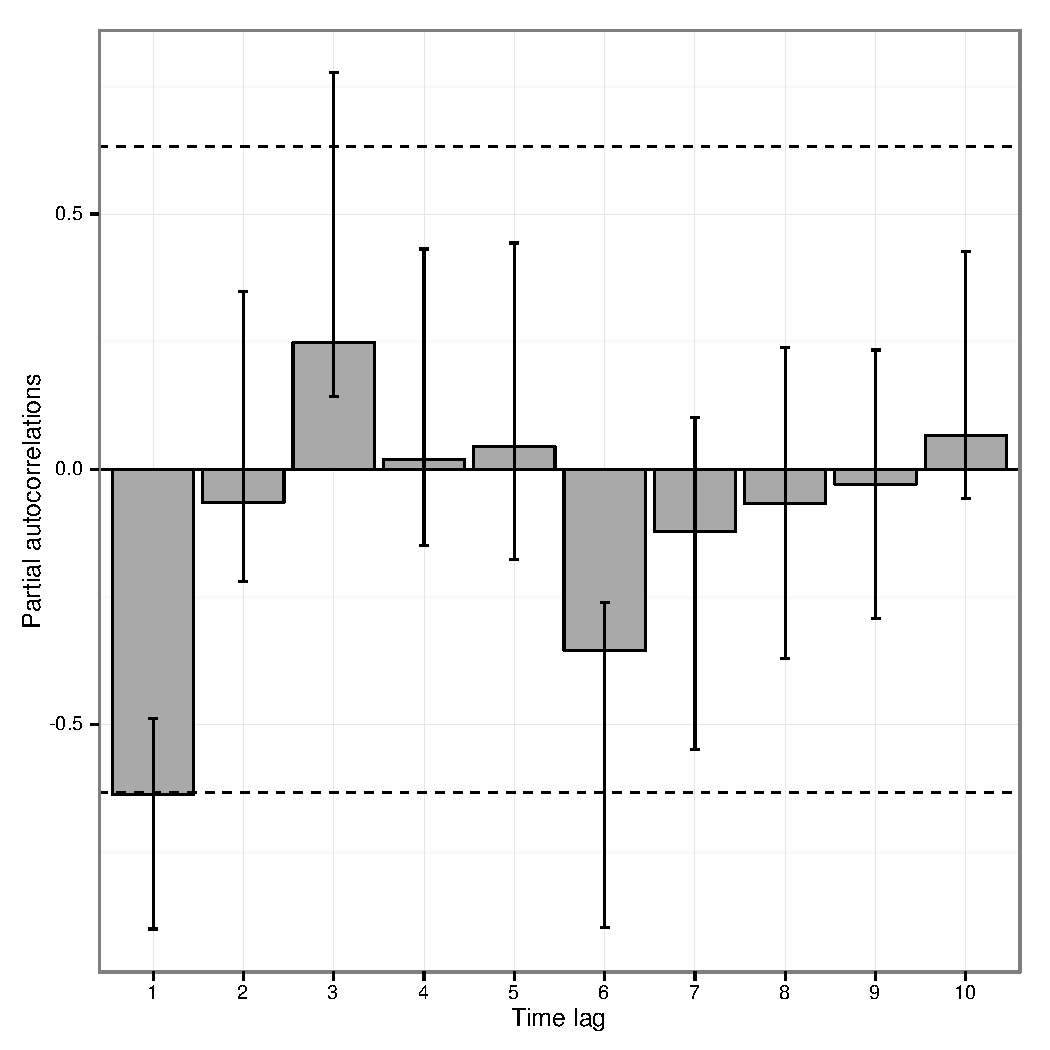
\includegraphics[width=65mm]{../White_Sea/dynamic_N_N1/boot_PRCF_Estuary_.pdf}

	\end{center}
	\end{minipage}
	%
	\hfil %Это пружинка отодвигающая рисунки друг от друга
	%
	\begin{minipage}[b]{.46\linewidth}
%Следующий рисунок - первый ряд справа %DUNGEON S_4 \ AB
	\begin{center}
	{\tiny Горелый верх}
		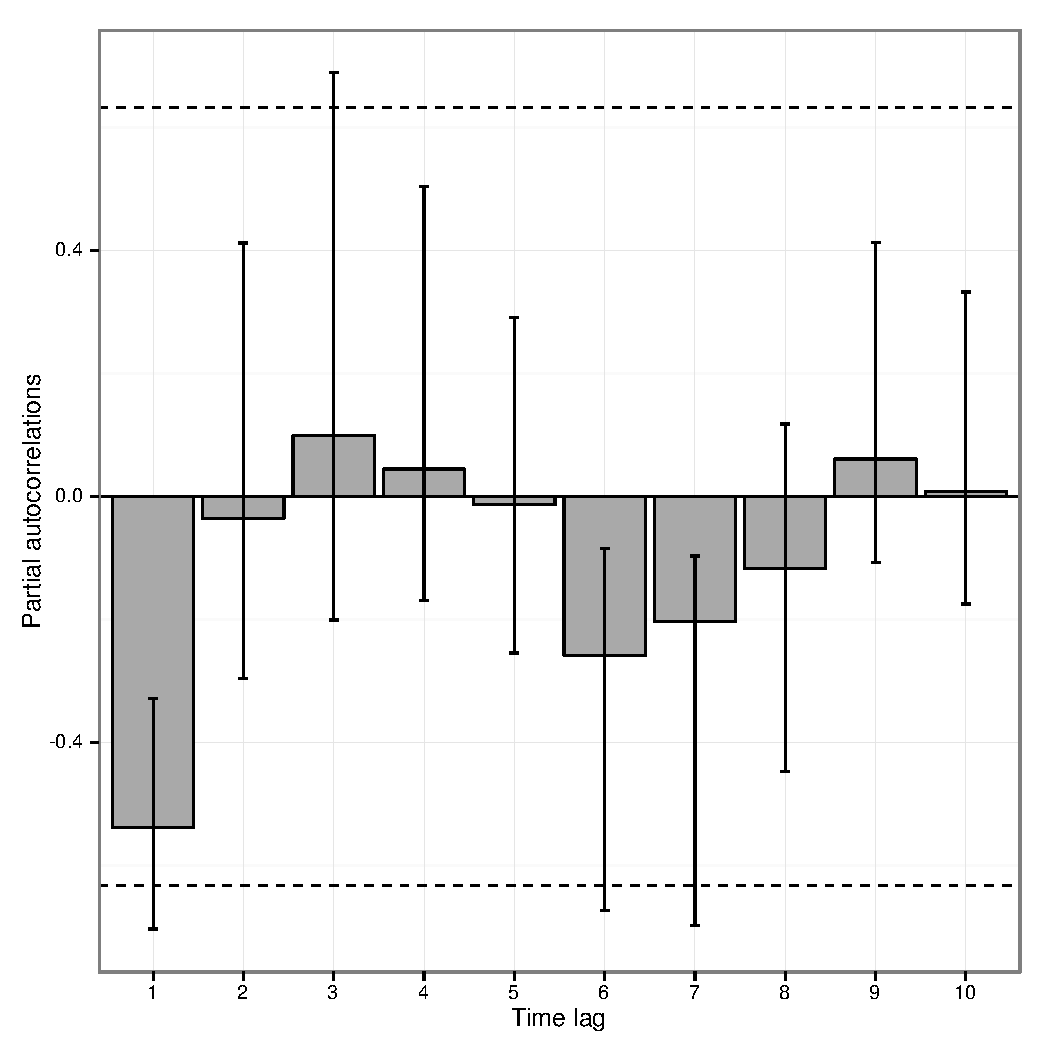
\includegraphics[width=65mm]{../White_Sea/dynamic_N_N1/boot_PRCF_Goreliy_high_.pdf}
	\end{center}
	\end{minipage}

%\smallskip


	\begin{minipage}[b]{.46\linewidth}
%Фигурка в первом ряду слева размер отведенный под весь этот объект \textendash 0.46 от ширины строки
%Параметр [b] означает, что выравнивание этих министраниц будет по нижнему краю
	\begin{center}
	{\tiny Горелый середина}
	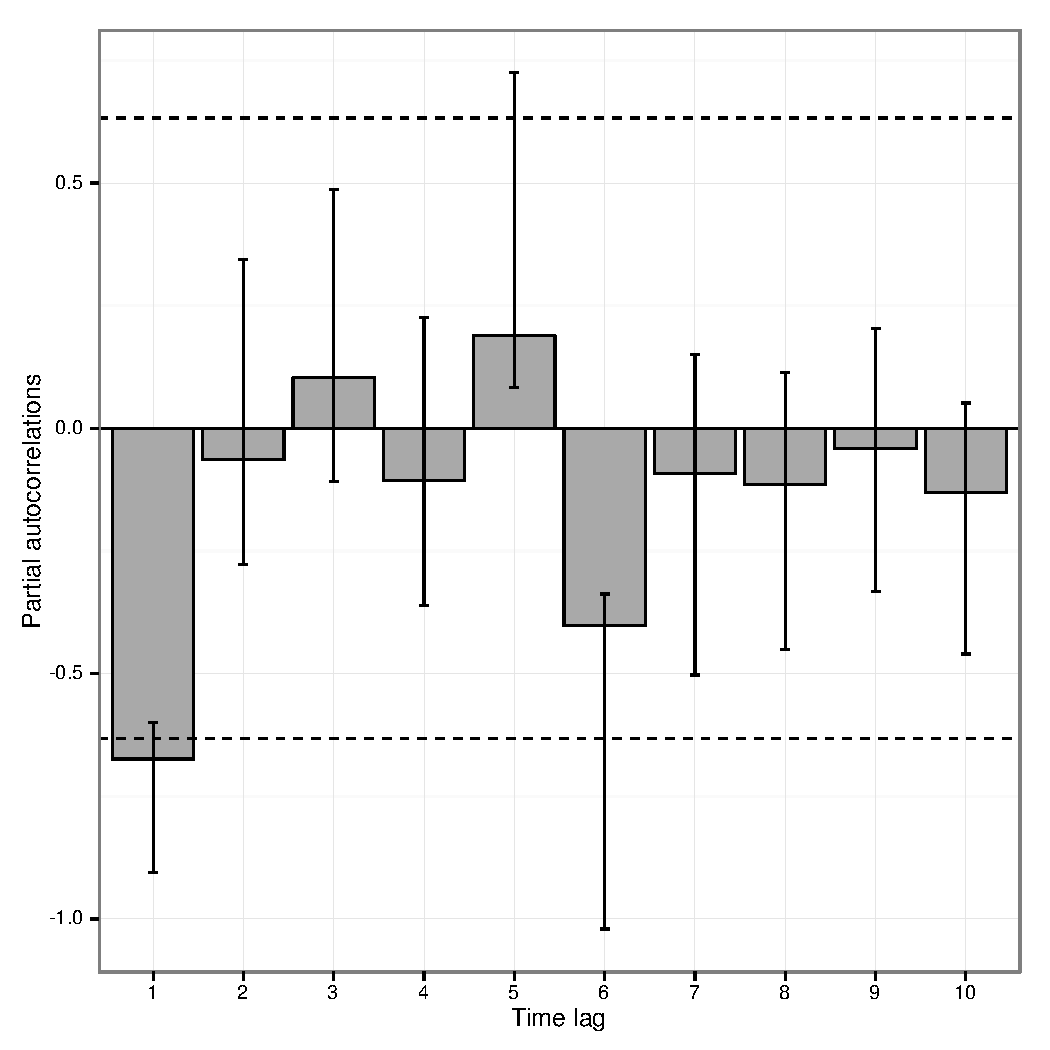
\includegraphics[width=65mm]{../White_Sea/dynamic_N_N1/boot_PRCF_Goreliy_middle_.pdf}
	\end{center}
	\end{minipage}
%
	\hfil %Это пружинка отодвигающая рисунки друг от друга
%
	\begin{minipage}[b]{.46\linewidth}
%Следующий рисунок - первый ряд справа %DUNGEON S_4 \ AB
	\begin{center}	
	{\tiny Горелый низ среднего}
	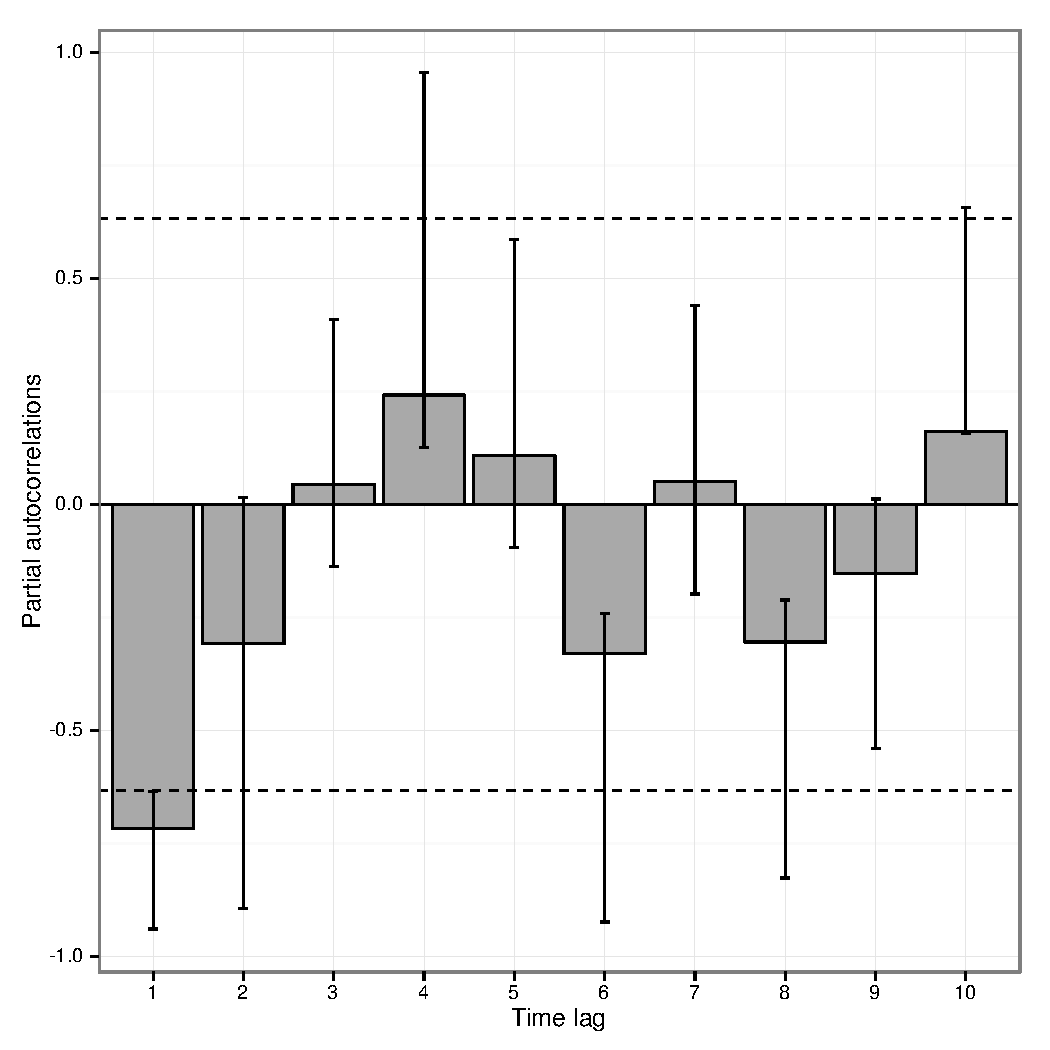
\includegraphics[width=65mm]{../White_Sea/dynamic_N_N1/boot_PRCF_Goreliy_midlow_.pdf}
	\end{center}
	\end{minipage}

%\smallskip

	\begin{minipage}[b]{.46\linewidth}
%Фигурка в первом ряду слева размер отведенный под весь этот объект \textendash 0.46 от ширины строки
%Параметр [b] означает, что выравнивание этих министраниц будет по нижнему краю
	\begin{center}
	{\tiny Горелый низ}
	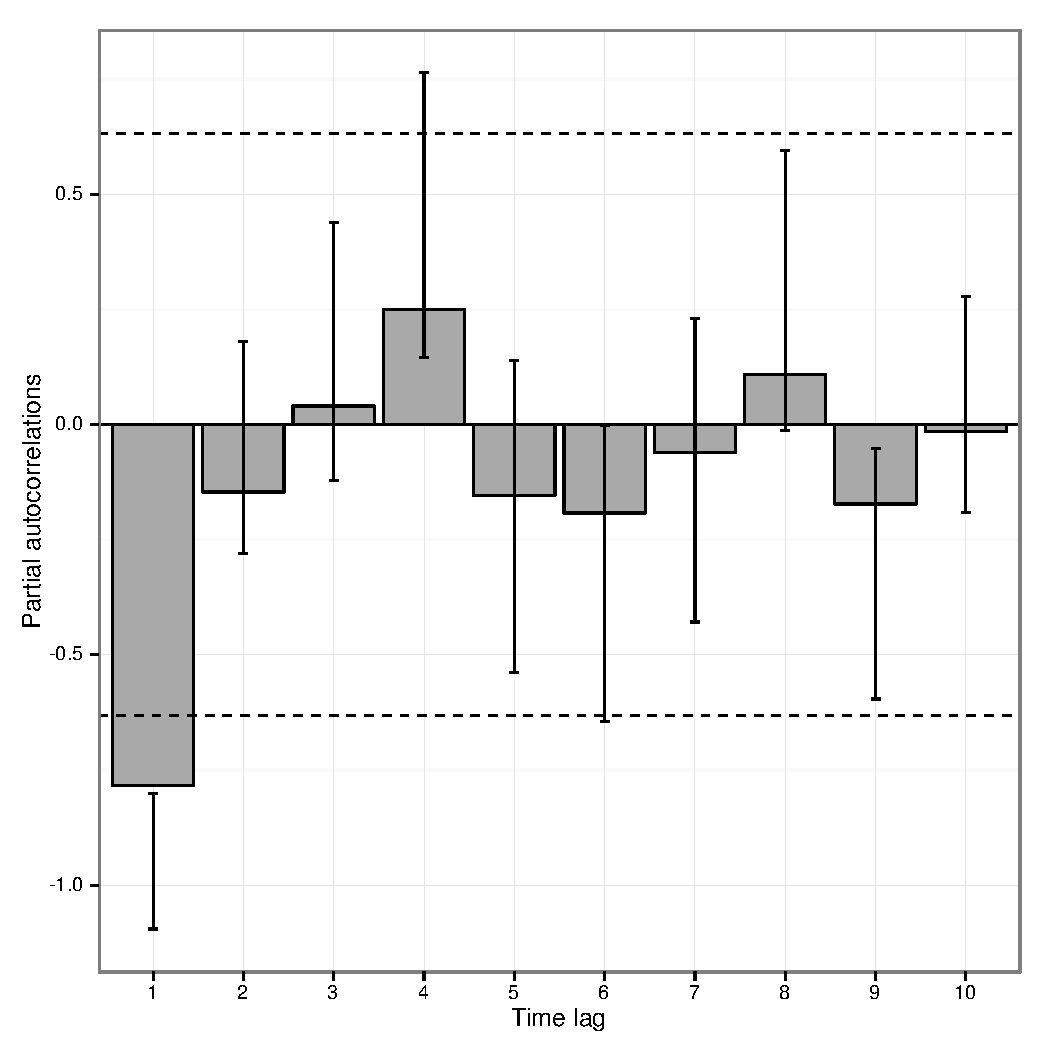
\includegraphics[width=65mm]{../White_Sea/dynamic_N_N1/boot_PRCF_Goreliy_low_.pdf}
	\end{center}
	\end{minipage}
%
	\hfil %Это пружинка отодвигающая рисунки друг от друга
%
	\begin{minipage}[b]{.46\linewidth}
%Следующий рисунок - первый ряд справа %DUNGEON S_4 \ AB
	\begin{center}
	{\tiny 2 разрез верхний пляж}
	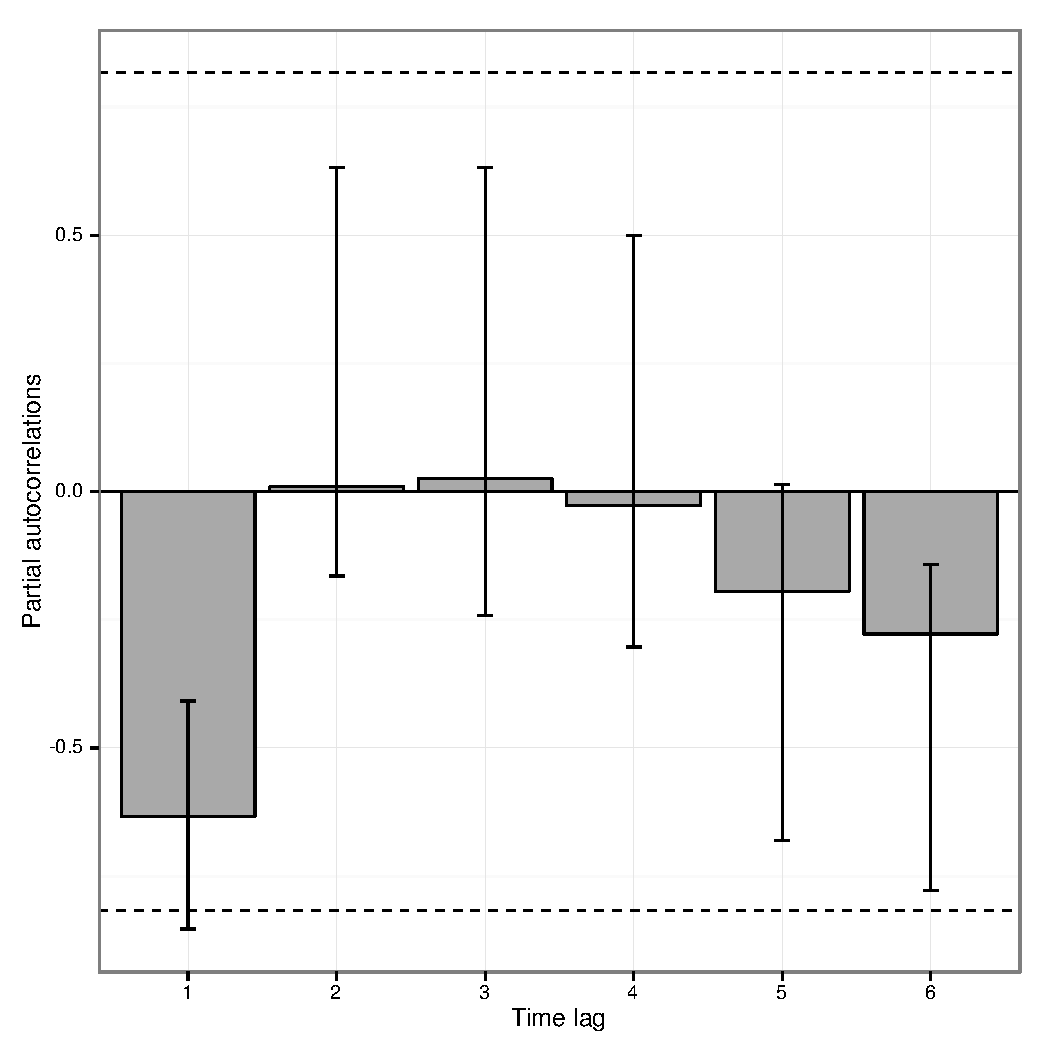
\includegraphics[width=65mm]{../White_Sea/dynamic_N_N1/boot_PRCF_razrez2_high_beatch_.pdf}
	\end{center}
	\end{minipage}

%\smallskip
	\caption{Частные автокорреляции численности {\it Macoma balthica} (без учета особей длиной менее 1 мм) в Кандалакшском заливе}
	\label{ris:boot_PRCF_Kandalaksha_N2}
	\end{figure}




	\begin{figure}[ht]
	
	\begin{minipage}[b]{.46\linewidth}
	%Фигурка в первом ряду слева размер отведенный под весь этот объект \textendash 0.46 от ширины строки
	%Параметр [b] означает, что выравнивание этих министраниц будет по нижнему краю
	\begin{center}
	{\tiny 2 разрез пояс фукоидов}
		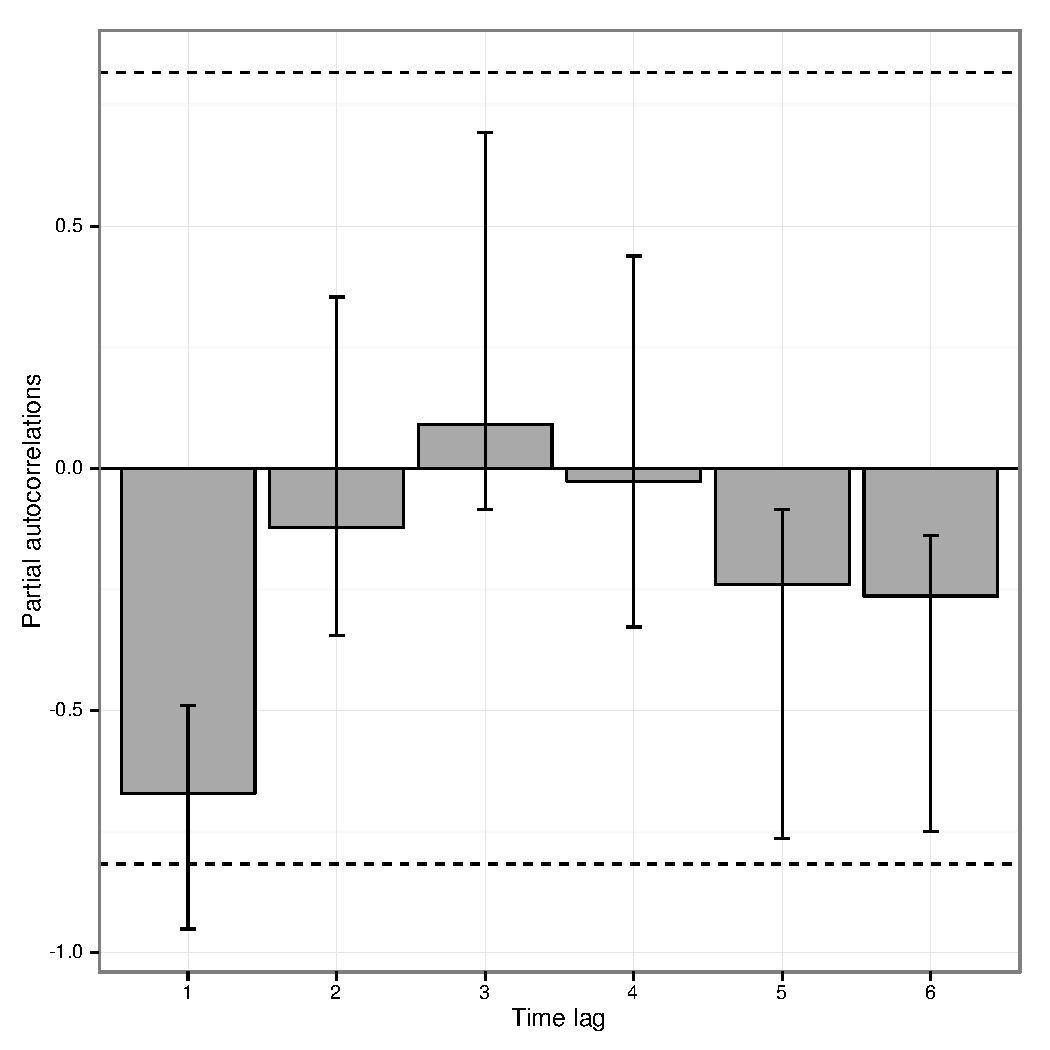
\includegraphics[width=65mm]{../White_Sea/dynamic_N_N1/boot_PRCF_razrez2_fucus_zone_.pdf}

	\end{center}
	\end{minipage}
	%
	\hfil %Это пружинка отодвигающая рисунки друг от друга
	%
	\begin{minipage}[b]{.46\linewidth}
%Следующий рисунок - первый ряд справа %DUNGEON S_4 \ AB
	\begin{center}
	{\tiny 2 разрез пояс зостеры}
		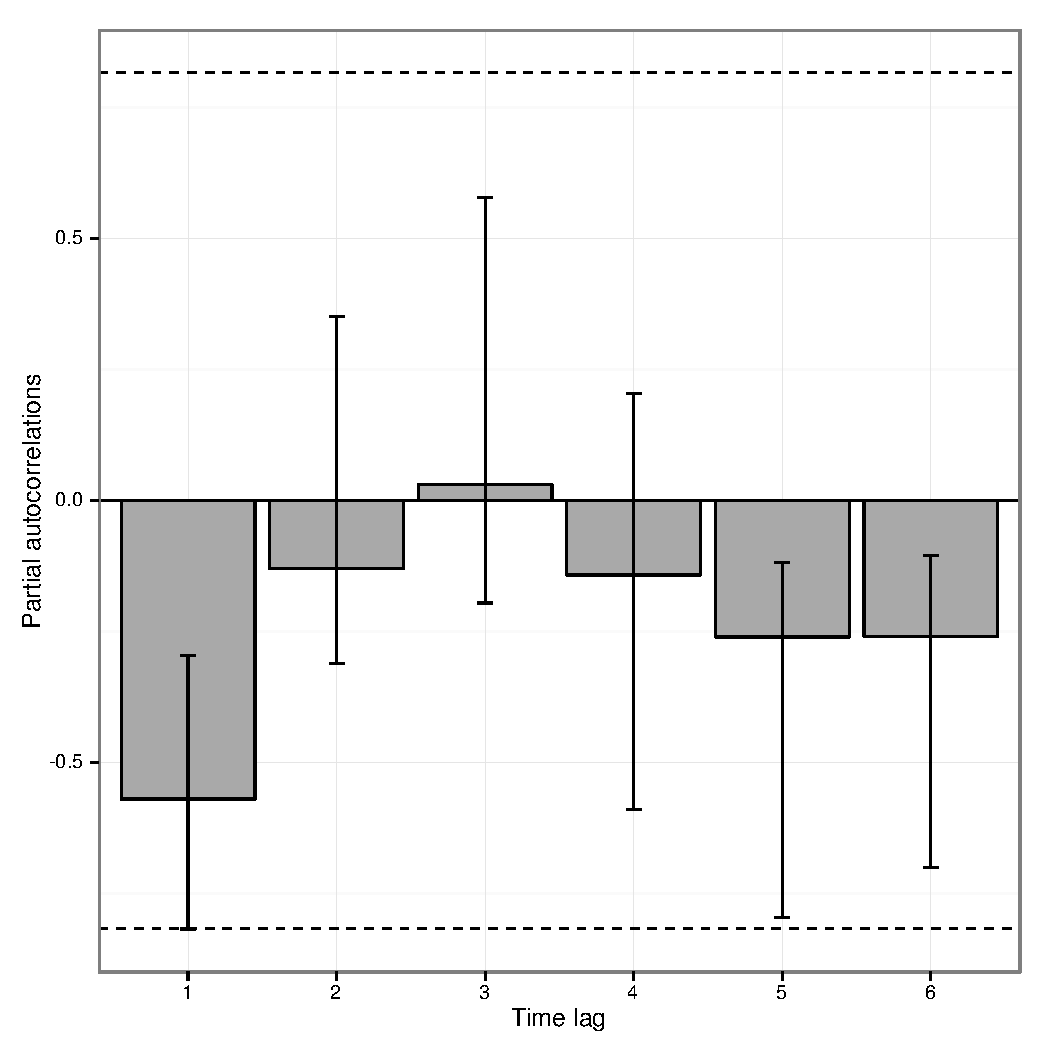
\includegraphics[width=65mm]{../White_Sea/dynamic_N_N1/boot_PRCF_razrez2_zostera_zone_.pdf}
	\end{center}
	\end{minipage}

%\smallskip


	\begin{minipage}[b]{.46\linewidth}
%Фигурка в первом ряду слева размер отведенный под весь этот объект \textendash 0.46 от ширины строки
%Параметр [b] означает, что выравнивание этих министраниц будет по нижнему краю
	\begin{center}
	{\tiny 2 разрез нижний пляж}
	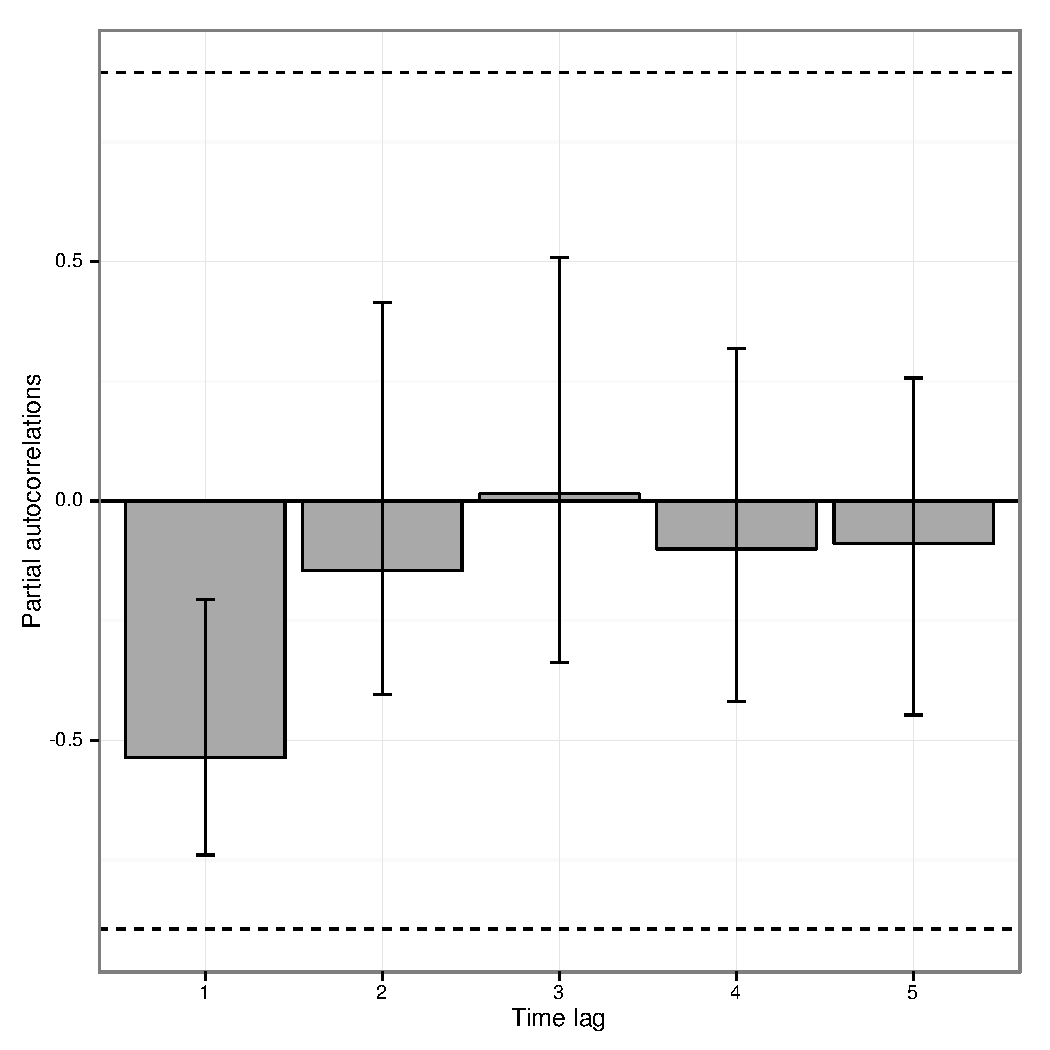
\includegraphics[width=65mm]{../White_Sea/dynamic_N_N1/boot_PRCF_razrez2_low_beatch_.pdf}
	\end{center}
	\end{minipage}
%
	\hfil %Это пружинка отодвигающая рисунки друг от друга
%
	\begin{minipage}[b]{.46\linewidth}
%Следующий рисунок - первый ряд справа %DUNGEON S_4 \ AB
	\begin{center}	
	{\tiny ЗРС}
	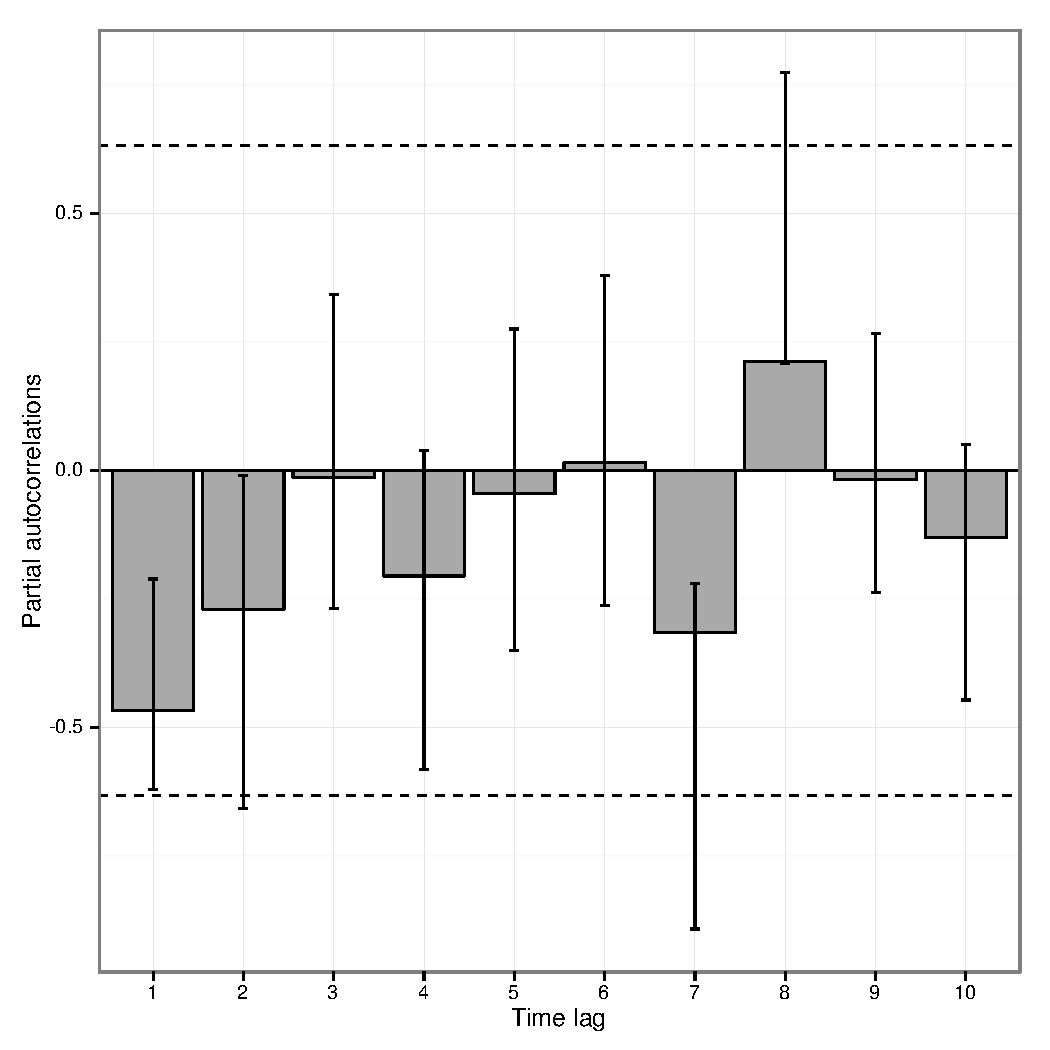
\includegraphics[width=65mm]{../White_Sea/dynamic_N_N1/boot_PRCF_ZRS_.pdf}
	\end{center}
	\end{minipage}

%\smallskip

	\begin{minipage}[b]{.46\linewidth}
%Фигурка в первом ряду слева размер отведенный под весь этот объект \textendash 0.46 от ширины строки
%Параметр [b] означает, что выравнивание этих министраниц будет по нижнему краю
	\begin{center}
	{\tiny Ломнишный}
	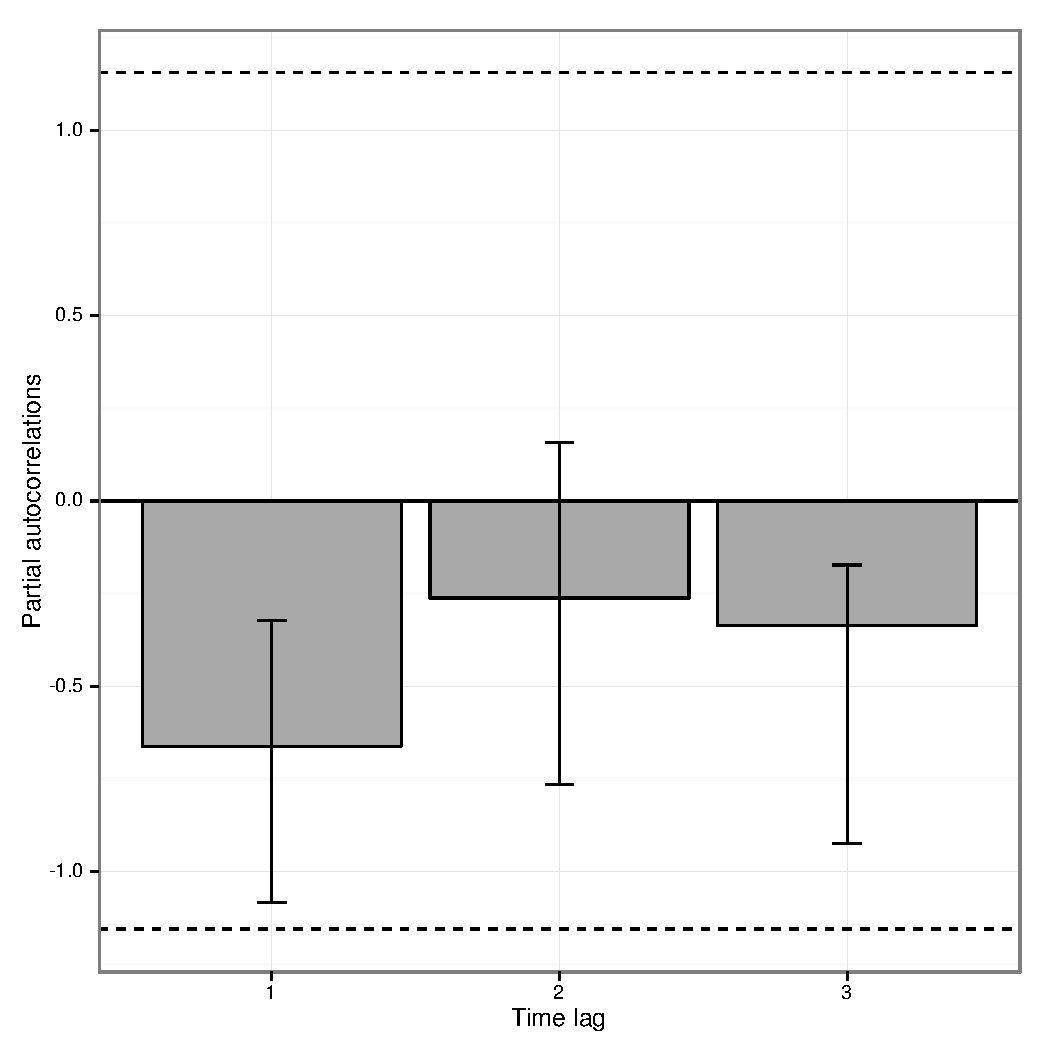
\includegraphics[width=65mm]{../White_Sea/dynamic_N_N1/boot_PRCF_Lomnishniy_.pdf}
	\end{center}
	\end{minipage}
%
	\hfil %Это пружинка отодвигающая рисунки друг от друга
%
	\begin{minipage}[b]{.46\linewidth}
%Следующий рисунок - первый ряд справа %DUNGEON S_4 \ AB
	\begin{center}
	{\tiny Южная губа}
	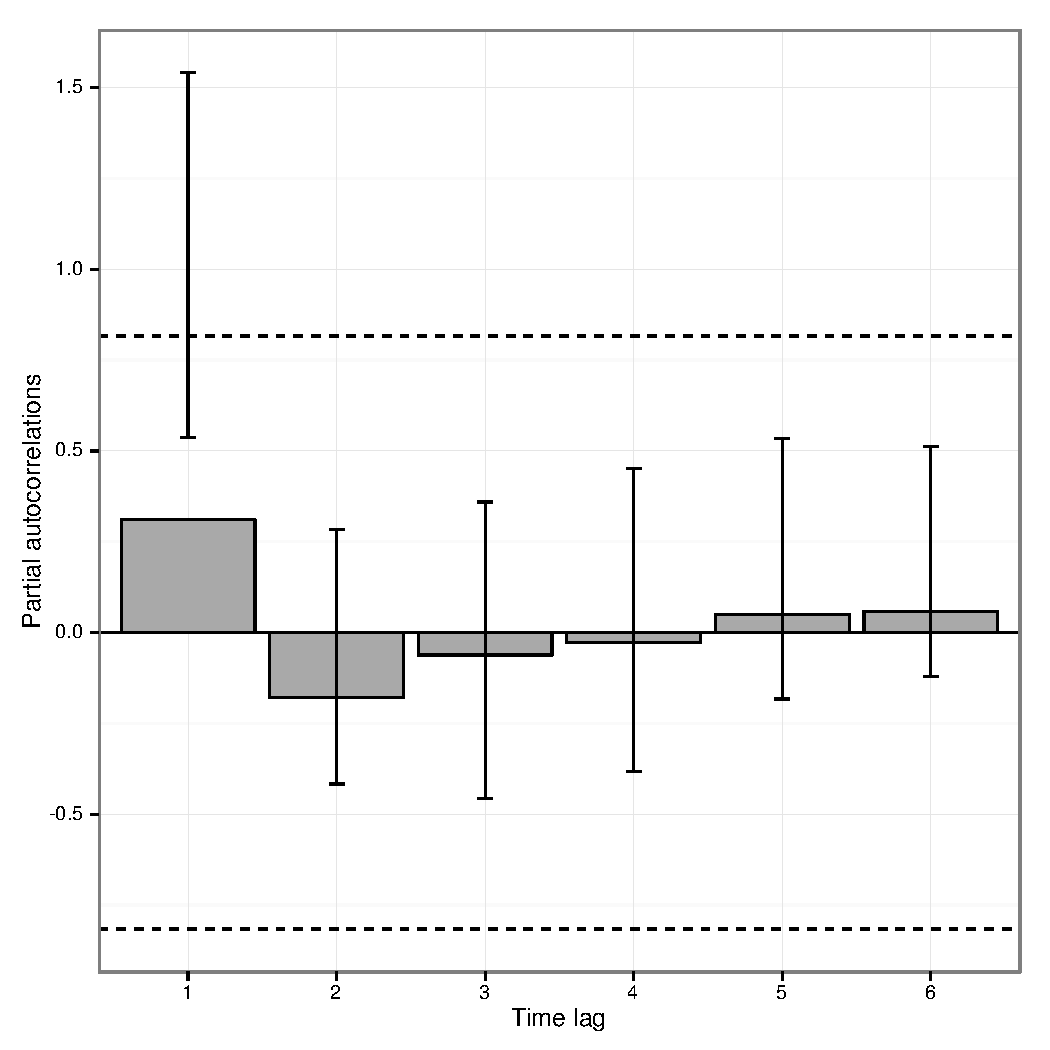
\includegraphics[width=65mm]{../White_Sea/dynamic_N_N1/boot_PRCF_YuG_.pdf}
	\end{center}
	\end{minipage}

%\smallskip
%	\caption{Динамика плотности поселений {\it Macoma balthica} в вершине Кандалакшского залива}
%	\label{ris:dynamic_Kandalaksha_all}
\begin{center}
Рисунок \ref{ris:boot_PRCF_Kandalaksha_N2}, продолжение. Частные автокорреляции численности {\it Macoma balthica} (без учета особей длиной менее 1 мм) в Кандалакшском заливе
\end{center}
	\end{figure}

	\begin{figure}[ht]
	
	\begin{minipage}[b]{.46\linewidth}
	%Фигурка в первом ряду слева размер отведенный под весь этот объект \textendash 0.46 от ширины строки
	%Параметр [b] означает, что выравнивание этих министраниц будет по нижнему краю
	\begin{center}
	{\tiny Эстуарий, детрендированные данные}
		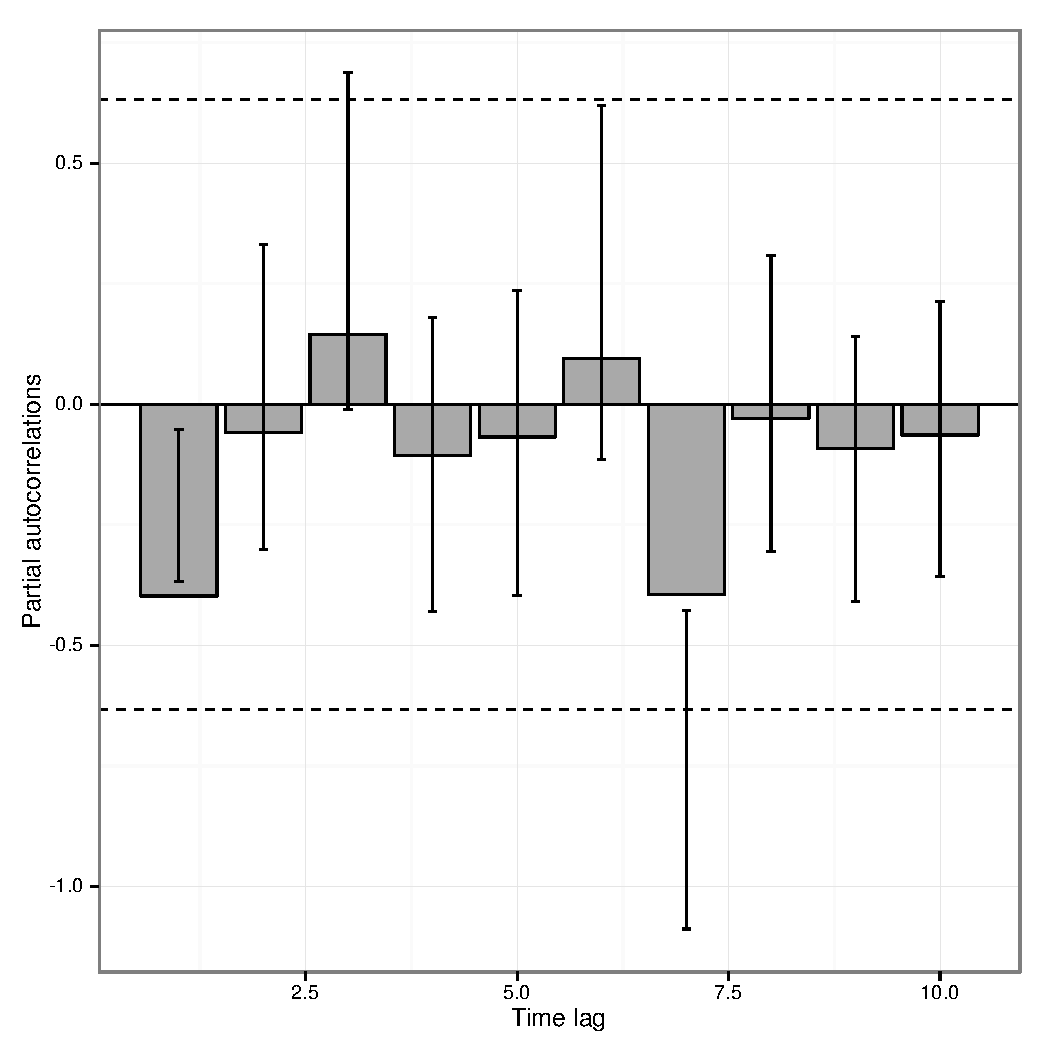
\includegraphics[width=65mm]{../White_Sea/dynamic_N_N1/boot_PRCF_Estuary_detrend.pdf}

	\end{center}
	\end{minipage}
	%
	\hfil %Это пружинка отодвигающая рисунки друг от друга
	%
	\begin{minipage}[b]{.46\linewidth}
%Следующий рисунок - первый ряд справа %DUNGEON S_4 \ AB
	\begin{center}
	{\tiny 2 разрез, фукусы. Детрендированные данные}
		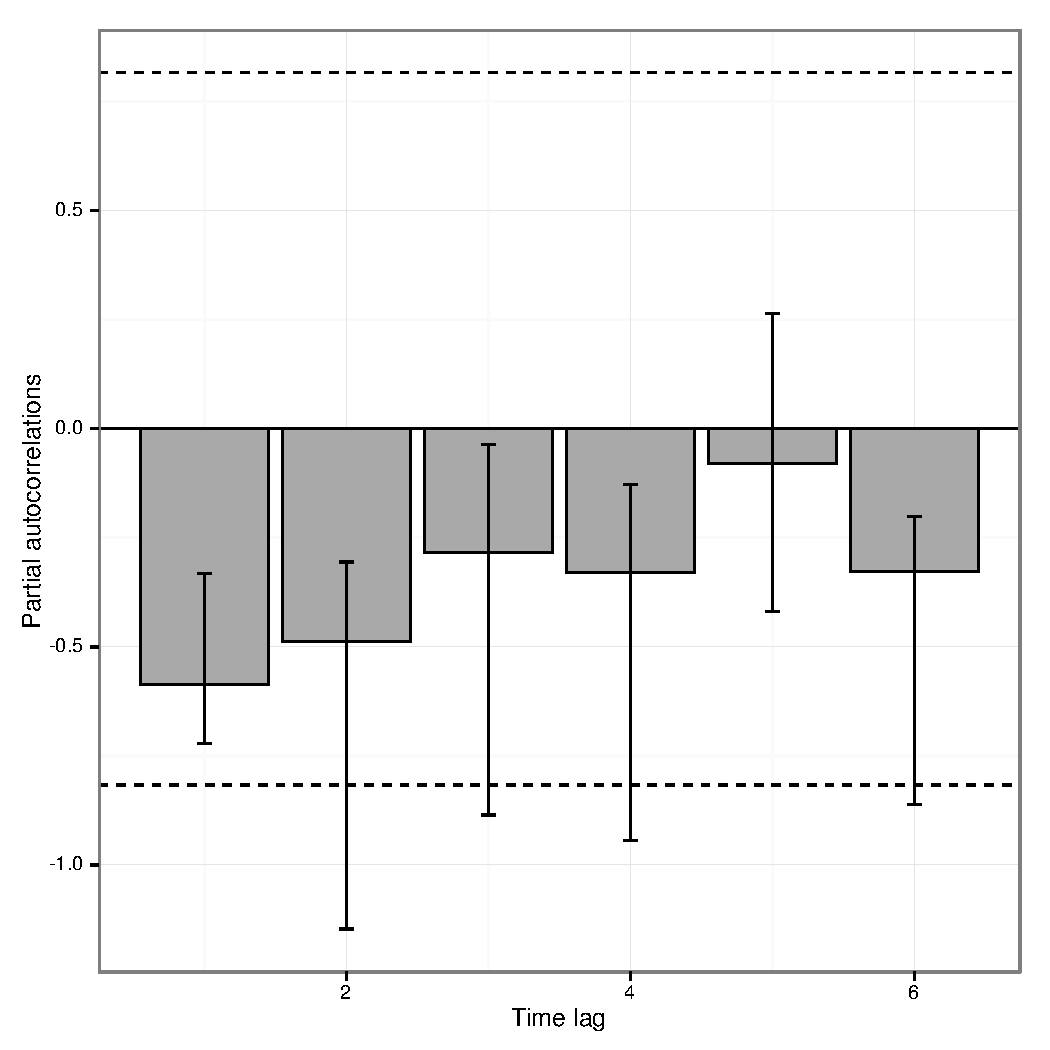
\includegraphics[width=65mm]{../White_Sea/dynamic_N_N1/boot_PRCF_razrez2_fucus_zone_detrend.pdf}
	\end{center}
	\end{minipage}

%\smallskip


	\begin{minipage}[b]{.46\linewidth}
%Фигурка в первом ряду слева размер отведенный под весь этот объект \textendash 0.46 от ширины строки
%Параметр [b] означает, что выравнивание этих министраниц будет по нижнему краю
	\begin{center}
	{\tiny 2 разрез, зостера. Детрендированные данные}
	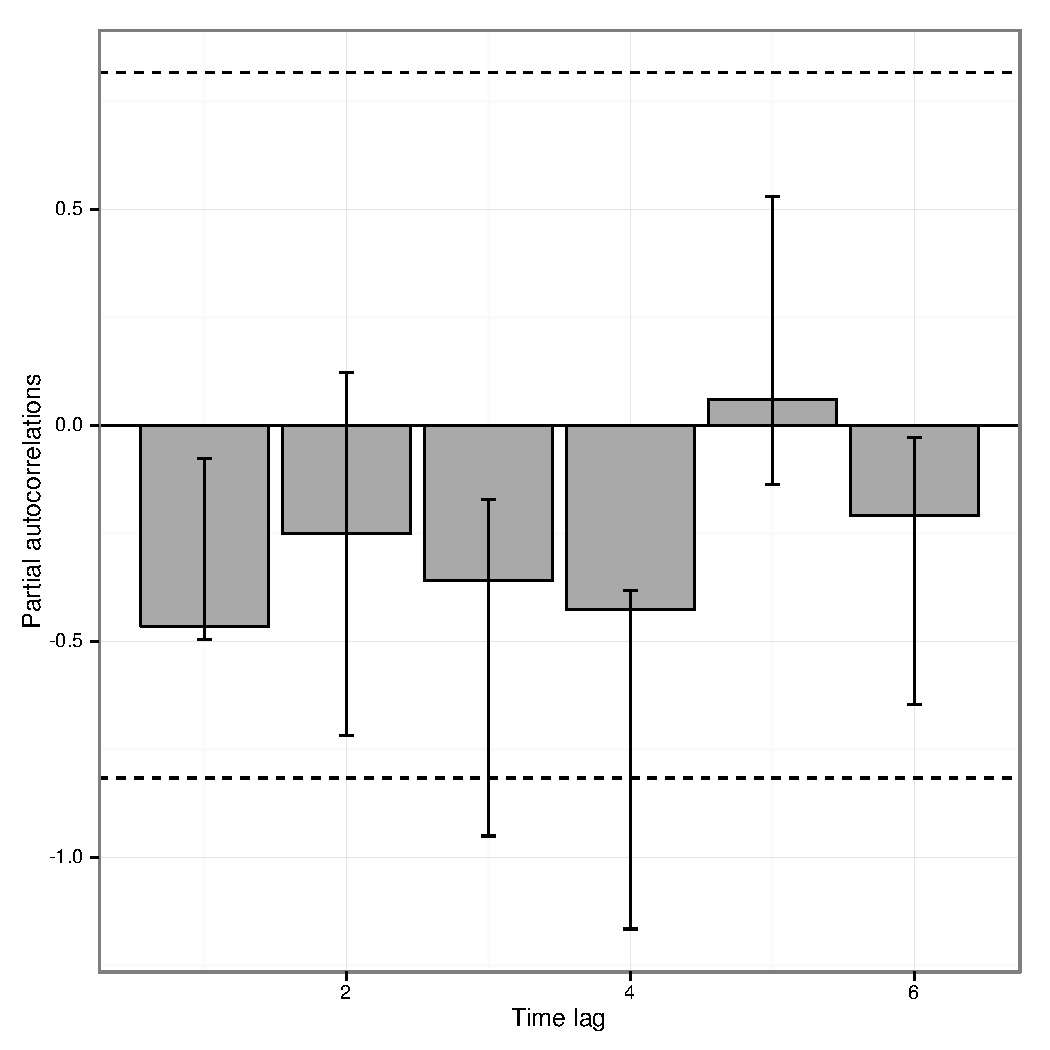
\includegraphics[width=65mm]{../White_Sea/dynamic_N_N1/boot_PRCF_razrez2_zostera_zone_detrend.pdf}
	\end{center}
	\end{minipage}
%
	\hfil %Это пружинка отодвигающая рисунки друг от друга
%
	\begin{minipage}[b]{.46\linewidth}
%Следующий рисунок - первый ряд справа %DUNGEON S_4 \ AB
	\begin{center}	
	{\tiny 2 разрез, нижний пляж. Детрендированные данные}
	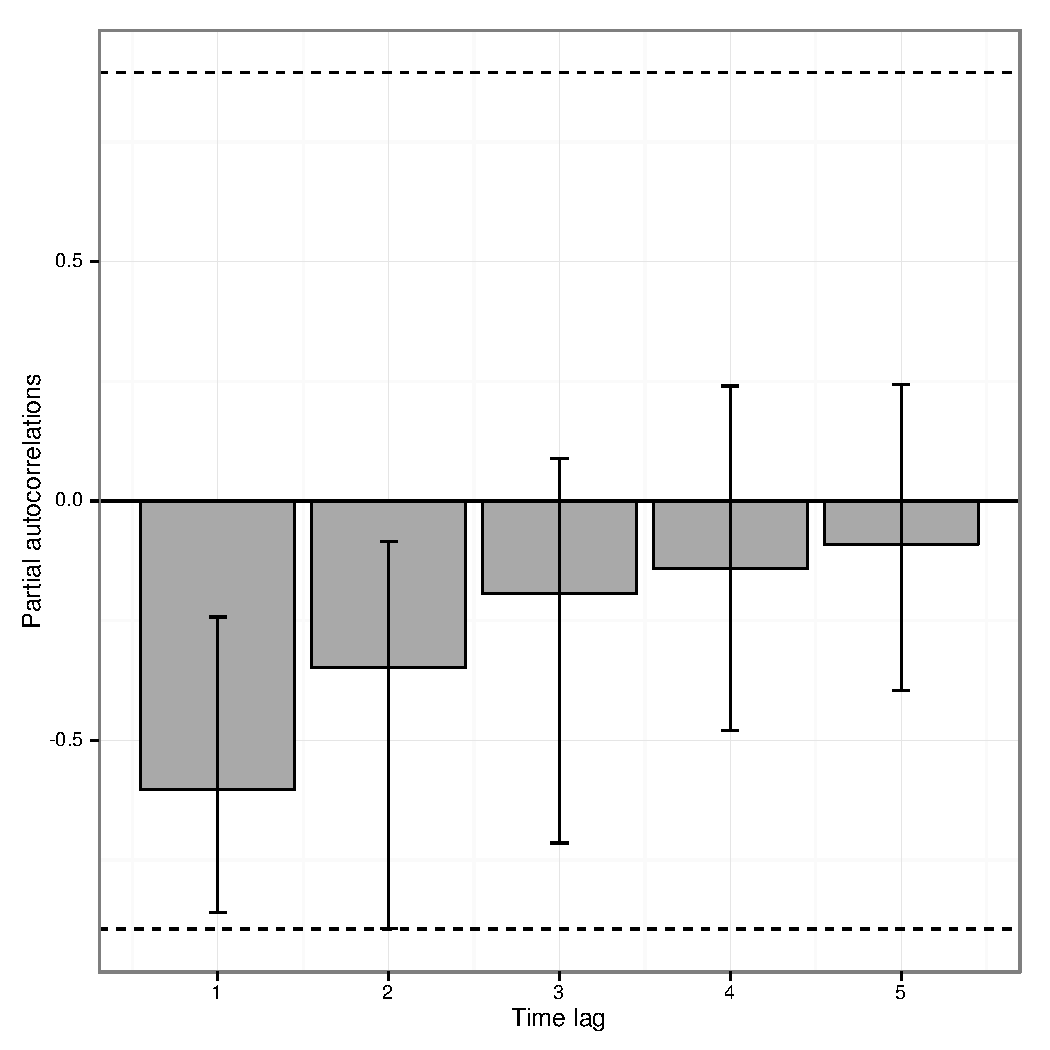
\includegraphics[width=65mm]{../White_Sea/dynamic_N_N1/boot_PRCF_razrez2_low_beatch_detrend.pdf}
	\end{center}
	\end{minipage}

%\smallskip

	\begin{minipage}[b]{.46\linewidth}
%Фигурка в первом ряду слева размер отведенный под весь этот объект \textendash 0.46 от ширины строки
%Параметр [b] означает, что выравнивание этих министраниц будет по нижнему краю
	\begin{center}
	{\tiny Южная губа. Детрендированные данные}
	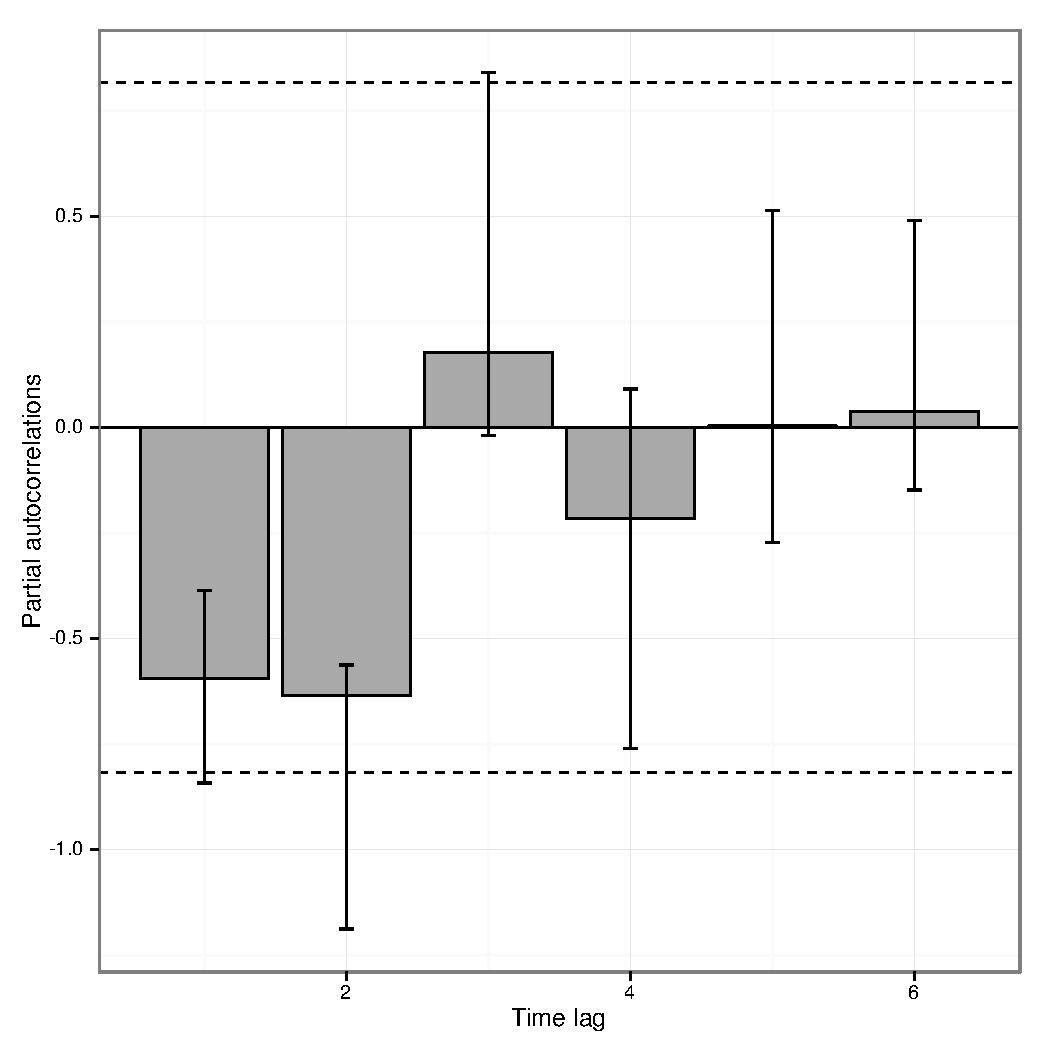
\includegraphics[width=65mm]{../White_Sea/dynamic_N_N1/boot_PRCF_YuG_detrend.pdf}
	\end{center}
	\end{minipage}
%
	\hfil %Это пружинка отодвигающая рисунки друг от друга
%
%	\begin{minipage}[b]{.46\linewidth}
%Следующий рисунок - первый ряд справа %DUNGEON S_4 \ AB
%	\begin{center}
%	{\tiny 2 разрез верхний пляж}
%	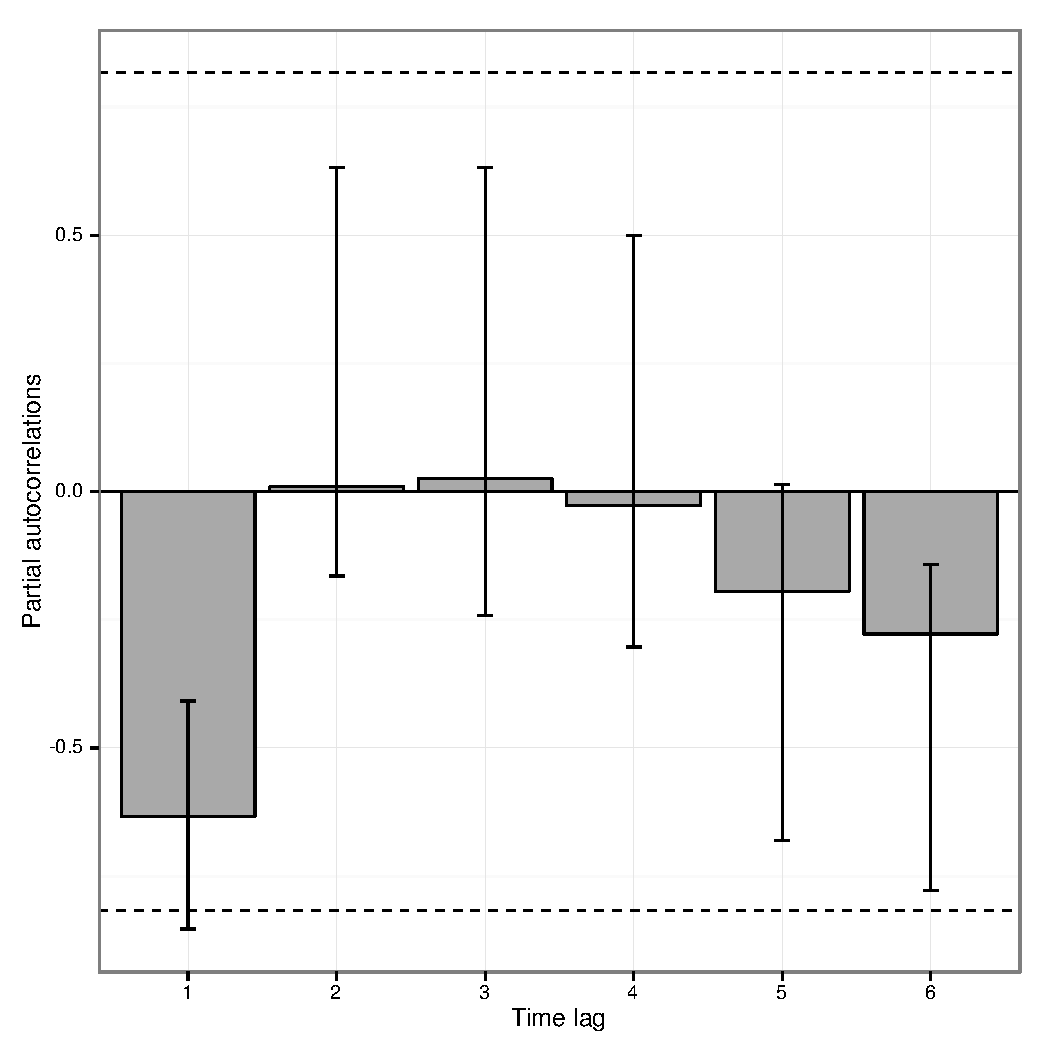
\includegraphics[width=65mm]{../White_Sea/dynamic_N_N1/boot_PRCF_razrez2_high_beatch_.pdf}
%	\end{center}
%	\end{minipage}

%\smallskip
	\caption{Частные автокорреляции численности {\it Macoma balthica} (без учета особей длиной менее 1 мм) в Кандалакшском заливе. Детрендированные данные.}
	\label{ris:boot_PRCF_Kandalaksha_N2_}
	\end{figure}


\end{document}
